%!TEX root = ../paper.tex



\def\AwfyBaseline{%
\begin{knitrout}
\definecolor{shadecolor}{rgb}{0.969, 0.969, 0.969}
% !TEX encoding = UTF-8 Unicode
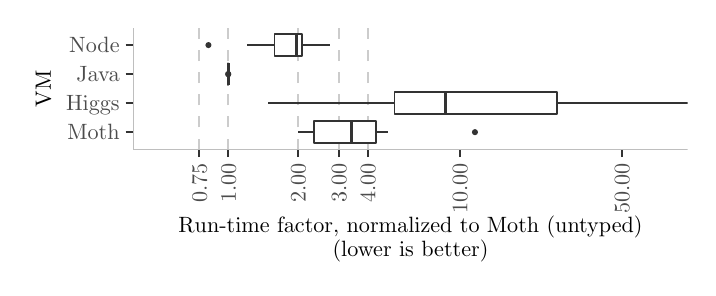
\begin{tikzpicture}[x=1pt,y=1pt]
\definecolor{fillColor}{RGB}{255,255,255}
\path[use as bounding box,fill=fillColor,fill opacity=0.00] (0,0) rectangle (238.49, 86.72);
\begin{scope}
\path[clip] ( 38.18, 42.66) rectangle (238.49, 86.72);
\definecolor{drawColor}{gray}{0.80}

\path[draw=drawColor,line width= 0.6pt,dash pattern=on 4pt off 4pt ,line join=round] ( 62.02, 42.66) -- ( 62.02, 86.72);

\path[draw=drawColor,line width= 0.6pt,dash pattern=on 4pt off 4pt ,line join=round] ( 72.47, 42.66) -- ( 72.47, 86.72);

\path[draw=drawColor,line width= 0.6pt,dash pattern=on 4pt off 4pt ,line join=round] ( 97.67, 42.66) -- ( 97.67, 86.72);

\path[draw=drawColor,line width= 0.6pt,dash pattern=on 4pt off 4pt ,line join=round] (112.40, 42.66) -- (112.40, 86.72);

\path[draw=drawColor,line width= 0.6pt,dash pattern=on 4pt off 4pt ,line join=round] (122.86, 42.66) -- (122.86, 86.72);
\definecolor{drawColor}{gray}{0.20}
\definecolor{fillColor}{gray}{0.20}

\path[draw=drawColor,line width= 0.4pt,line join=round,line cap=round,fill=fillColor] (161.62, 48.96) circle (  0.89);

\path[draw=drawColor,line width= 0.6pt,line join=round] (125.82, 48.96) -- (130.15, 48.96);

\path[draw=drawColor,line width= 0.6pt,line join=round] (103.56, 48.96) -- ( 97.73, 48.96);
\definecolor{fillColor}{RGB}{255,255,255}

\path[draw=drawColor,line width= 0.6pt,line join=round,line cap=round,fill=fillColor] (125.82, 45.02) --
	(103.56, 45.02) --
	(103.56, 52.89) --
	(125.82, 52.89) --
	(125.82, 45.02) --
	cycle;

\path[draw=drawColor,line width= 1.1pt,line join=round] (116.85, 45.02) -- (116.85, 52.89);

\path[draw=drawColor,line width= 0.6pt,line join=round] (191.21, 59.45) -- (238.49, 59.45);

\path[draw=drawColor,line width= 0.6pt,line join=round] (132.56, 59.45) -- ( 86.96, 59.45);

\path[draw=drawColor,line width= 0.6pt,line join=round,line cap=round,fill=fillColor] (191.21, 55.51) --
	(132.56, 55.51) --
	(132.56, 63.38) --
	(191.21, 63.38) --
	(191.21, 55.51) --
	cycle;

\path[draw=drawColor,line width= 1.1pt,line join=round] (150.88, 55.51) -- (150.88, 63.38);
\definecolor{fillColor}{gray}{0.20}

\path[draw=drawColor,line width= 0.4pt,line join=round,line cap=round,fill=fillColor] ( 72.47, 69.94) circle (  0.89);

\path[draw=drawColor,line width= 0.4pt,line join=round,line cap=round,fill=fillColor] ( 72.47, 69.94) circle (  0.89);

\path[draw=drawColor,line width= 0.6pt,line join=round] ( 72.47, 69.94) -- ( 72.47, 69.94);

\path[draw=drawColor,line width= 0.6pt,line join=round] ( 72.47, 69.94) -- ( 72.47, 69.94);
\definecolor{fillColor}{RGB}{255,255,255}

\path[draw=drawColor,line width= 0.6pt,line join=round,line cap=round,fill=fillColor] ( 72.47, 66.00) --
	( 72.47, 66.00) --
	( 72.47, 73.87) --
	( 72.47, 73.87) --
	( 72.47, 66.00) --
	cycle;

\path[draw=drawColor,line width= 1.1pt,line join=round] ( 72.47, 66.00) -- ( 72.47, 73.87);
\definecolor{fillColor}{gray}{0.20}

\path[draw=drawColor,line width= 0.4pt,line join=round,line cap=round,fill=fillColor] ( 65.32, 80.43) circle (  0.89);

\path[draw=drawColor,line width= 0.6pt,line join=round] ( 99.20, 80.43) -- (109.14, 80.43);

\path[draw=drawColor,line width= 0.6pt,line join=round] ( 89.18, 80.43) -- ( 79.19, 80.43);
\definecolor{fillColor}{RGB}{255,255,255}

\path[draw=drawColor,line width= 0.6pt,line join=round,line cap=round,fill=fillColor] ( 99.20, 76.50) --
	( 89.18, 76.50) --
	( 89.18, 84.36) --
	( 99.20, 84.36) --
	( 99.20, 76.50) --
	cycle;

\path[draw=drawColor,line width= 1.1pt,line join=round] ( 97.20, 76.50) -- ( 97.20, 84.36);
\end{scope}
\begin{scope}
\path[clip] (  0.00,  0.00) rectangle (238.49, 86.72);
\definecolor{drawColor}{RGB}{190,190,190}

\path[draw=drawColor,line width= 0.6pt,line join=round] ( 38.18, 42.66) --
	( 38.18, 86.72);
\end{scope}
\begin{scope}
\path[clip] (  0.00,  0.00) rectangle (238.49, 86.72);
\definecolor{drawColor}{gray}{0.30}

\node[text=drawColor,anchor=base east,inner sep=0pt, outer sep=0pt, scale=  0.80] at ( 33.23, 46.20) {Moth};

\node[text=drawColor,anchor=base east,inner sep=0pt, outer sep=0pt, scale=  0.80] at ( 33.23, 56.69) {Higgs};

\node[text=drawColor,anchor=base east,inner sep=0pt, outer sep=0pt, scale=  0.80] at ( 33.23, 67.18) {Java};

\node[text=drawColor,anchor=base east,inner sep=0pt, outer sep=0pt, scale=  0.80] at ( 33.23, 77.67) {Node};
\end{scope}
\begin{scope}
\path[clip] (  0.00,  0.00) rectangle (238.49, 86.72);
\definecolor{drawColor}{gray}{0.20}

\path[draw=drawColor,line width= 0.6pt,line join=round] ( 35.43, 48.96) --
	( 38.18, 48.96);

\path[draw=drawColor,line width= 0.6pt,line join=round] ( 35.43, 59.45) --
	( 38.18, 59.45);

\path[draw=drawColor,line width= 0.6pt,line join=round] ( 35.43, 69.94) --
	( 38.18, 69.94);

\path[draw=drawColor,line width= 0.6pt,line join=round] ( 35.43, 80.43) --
	( 38.18, 80.43);
\end{scope}
\begin{scope}
\path[clip] (  0.00,  0.00) rectangle (238.49, 86.72);
\definecolor{drawColor}{RGB}{190,190,190}

\path[draw=drawColor,line width= 0.6pt,line join=round] ( 38.18, 42.66) --
	(238.49, 42.66);
\end{scope}
\begin{scope}
\path[clip] (  0.00,  0.00) rectangle (238.49, 86.72);
\definecolor{drawColor}{gray}{0.20}

\path[draw=drawColor,line width= 0.6pt,line join=round] ( 62.02, 39.91) --
	( 62.02, 42.66);

\path[draw=drawColor,line width= 0.6pt,line join=round] ( 72.47, 39.91) --
	( 72.47, 42.66);

\path[draw=drawColor,line width= 0.6pt,line join=round] ( 97.67, 39.91) --
	( 97.67, 42.66);

\path[draw=drawColor,line width= 0.6pt,line join=round] (112.40, 39.91) --
	(112.40, 42.66);

\path[draw=drawColor,line width= 0.6pt,line join=round] (122.86, 39.91) --
	(122.86, 42.66);

\path[draw=drawColor,line width= 0.6pt,line join=round] (156.16, 39.91) --
	(156.16, 42.66);

\path[draw=drawColor,line width= 0.6pt,line join=round] (214.65, 39.91) --
	(214.65, 42.66);
\end{scope}
\begin{scope}
\path[clip] (  0.00,  0.00) rectangle (238.49, 86.72);
\definecolor{drawColor}{gray}{0.30}

\node[text=drawColor,rotate= 90.00,anchor=base east,inner sep=0pt, outer sep=0pt, scale=  0.80] at ( 64.77, 37.71) {0.75};

\node[text=drawColor,rotate= 90.00,anchor=base east,inner sep=0pt, outer sep=0pt, scale=  0.80] at ( 75.23, 37.71) {1.00};

\node[text=drawColor,rotate= 90.00,anchor=base east,inner sep=0pt, outer sep=0pt, scale=  0.80] at (100.42, 37.71) {2.00};

\node[text=drawColor,rotate= 90.00,anchor=base east,inner sep=0pt, outer sep=0pt, scale=  0.80] at (115.16, 37.71) {3.00};

\node[text=drawColor,rotate= 90.00,anchor=base east,inner sep=0pt, outer sep=0pt, scale=  0.80] at (125.61, 37.71) {4.00};

\node[text=drawColor,rotate= 90.00,anchor=base east,inner sep=0pt, outer sep=0pt, scale=  0.80] at (158.91, 37.71) {10.00};

\node[text=drawColor,rotate= 90.00,anchor=base east,inner sep=0pt, outer sep=0pt, scale=  0.80] at (217.40, 37.71) {50.00};
\end{scope}
\begin{scope}
\path[clip] (  0.00,  0.00) rectangle (238.49, 86.72);
\definecolor{drawColor}{RGB}{0,0,0}

\node[text=drawColor,anchor=base,inner sep=0pt, outer sep=0pt, scale=  0.80] at (138.33, 12.73) {Run-time factor, normalized to Moth (untyped)};

\node[text=drawColor,anchor=base,inner sep=0pt, outer sep=0pt, scale=  0.80] at (138.33,  4.09) {(lower is better)};
\end{scope}
\begin{scope}
\path[clip] (  0.00,  0.00) rectangle (238.49, 86.72);
\definecolor{drawColor}{RGB}{0,0,0}

\node[text=drawColor,rotate= 90.00,anchor=base,inner sep=0pt, outer sep=0pt, scale=  0.80] at (  8.36, 64.69) {VM};
\end{scope}
\end{tikzpicture}


\end{knitrout}
}%



\newcommand{\OverheadNodeGMeanX}{1.8x\xspace}
\newcommand{\OverheadNodeMinX}{0.8x\xspace}
\newcommand{\OverheadNodeMaxX}{2.7x\xspace}

\newcommand{\OverheadMothGMeanX}{2.3x\xspace}
\newcommand{\OverheadMothMinX}{0.9x\xspace}
\newcommand{\OverheadMothMaxX}{4.1x\xspace}

\newcommand{\OverheadMothNodeGMeanX}{1.3x\xspace}
\newcommand{\OverheadMothNodeMinX}{0.8x\xspace}
\newcommand{\OverheadMothNodeMaxX}{2.1x\xspace}

\newcommand{\OverheadMothNodeGMeanP}{28\%\xspace}
\newcommand{\OverheadMothNodeMinP}{-17\%\xspace}
\newcommand{\OverheadMothNodeMaxP}{115\%\xspace}

\newcommand{\OverheadHiggsGMeanX}{13.8x\xspace}
\newcommand{\OverheadHiggsMinX}{1.5x\xspace}
\newcommand{\OverheadHiggsMaxX}{168.9x\xspace}



